\chapter{Konstrukcja}
	\section{Wybór mikrokontrolera}
		W przypadku robota autonomicznego istotną jego częścią jest jednostka logiczna, która nim steruje. Powinna być wystarczająco wydajna aby umożliwić szybkie podejmowanie decyzji na podstawie odczytów z czujników oraz stanu wewnętrznego robota. W przypadku braku zewnętrznego sterowania przez operatora, robot sam powinien unikać kolizji oraz decydować o kierunku poruszania się.
		
		Obecnie dostępnych jest wiele rodzajów mikrokontrolerów, a konkurencyjność zapewnia niskie ceny zakupu. To sprawia, że są one w zasięgu finansowym przeciętnego człowieka. Najbardziej rozpowszechnioną platformą jest seria Arduino \cite{arduinoFramework}. Posiada ona dużą ilość użytkowników i dzięki temu można łatwo uzyskać wsparcie w przypadku problemu z platformą. Przykładową gotową płytką z 8-bitowym procesorem ATmega2560 jest Arduino Mega \ref{fig:mikrokontrolery}. Posiada zegar o maksymalnej częstotliwości 16Mhz, 54 piny cyfrowe (w tym 15 PWM i 6 wspierających przerwania), 16 pinów analogowych i 6 timerów. Cena w przypadku nieoryginalnej wersji płytki wynosi około 7\$ (28zł)
		
		Kolejnym przykładem rodziny mikrokontrolerów z dużym wsparciem użytkowników jest Raspberry Pi. Przykładową płytką jest Raspberry Pi 4 model B \ref{fig:mikrokontrolery}. Posiada 4-rdzeniowy, 64-bitowy procesor o taktowaniu GHz, od 1 do 4GB pamięci RAM oraz 40 pinów cyfrowych. Zaletą tej płytki jest jej wysoka wydajność i możliwość wgrania pełnoprawnego systemu operacyjnego. Przykładem może być system operacyjny Rasbian \cite{raspbian}. Jest to wersja Linuxa podobna do systemu Debian. Minusem jest cena która dla najnowszego modelu wynosi około 50\$ (200zł) natomiast dla starszej wersji około 40\$ (160zł).
	
		\begin{figure}[h]
			\centering
			\begin{tabular}{@{}ll@{}}
				a) & b) \\
				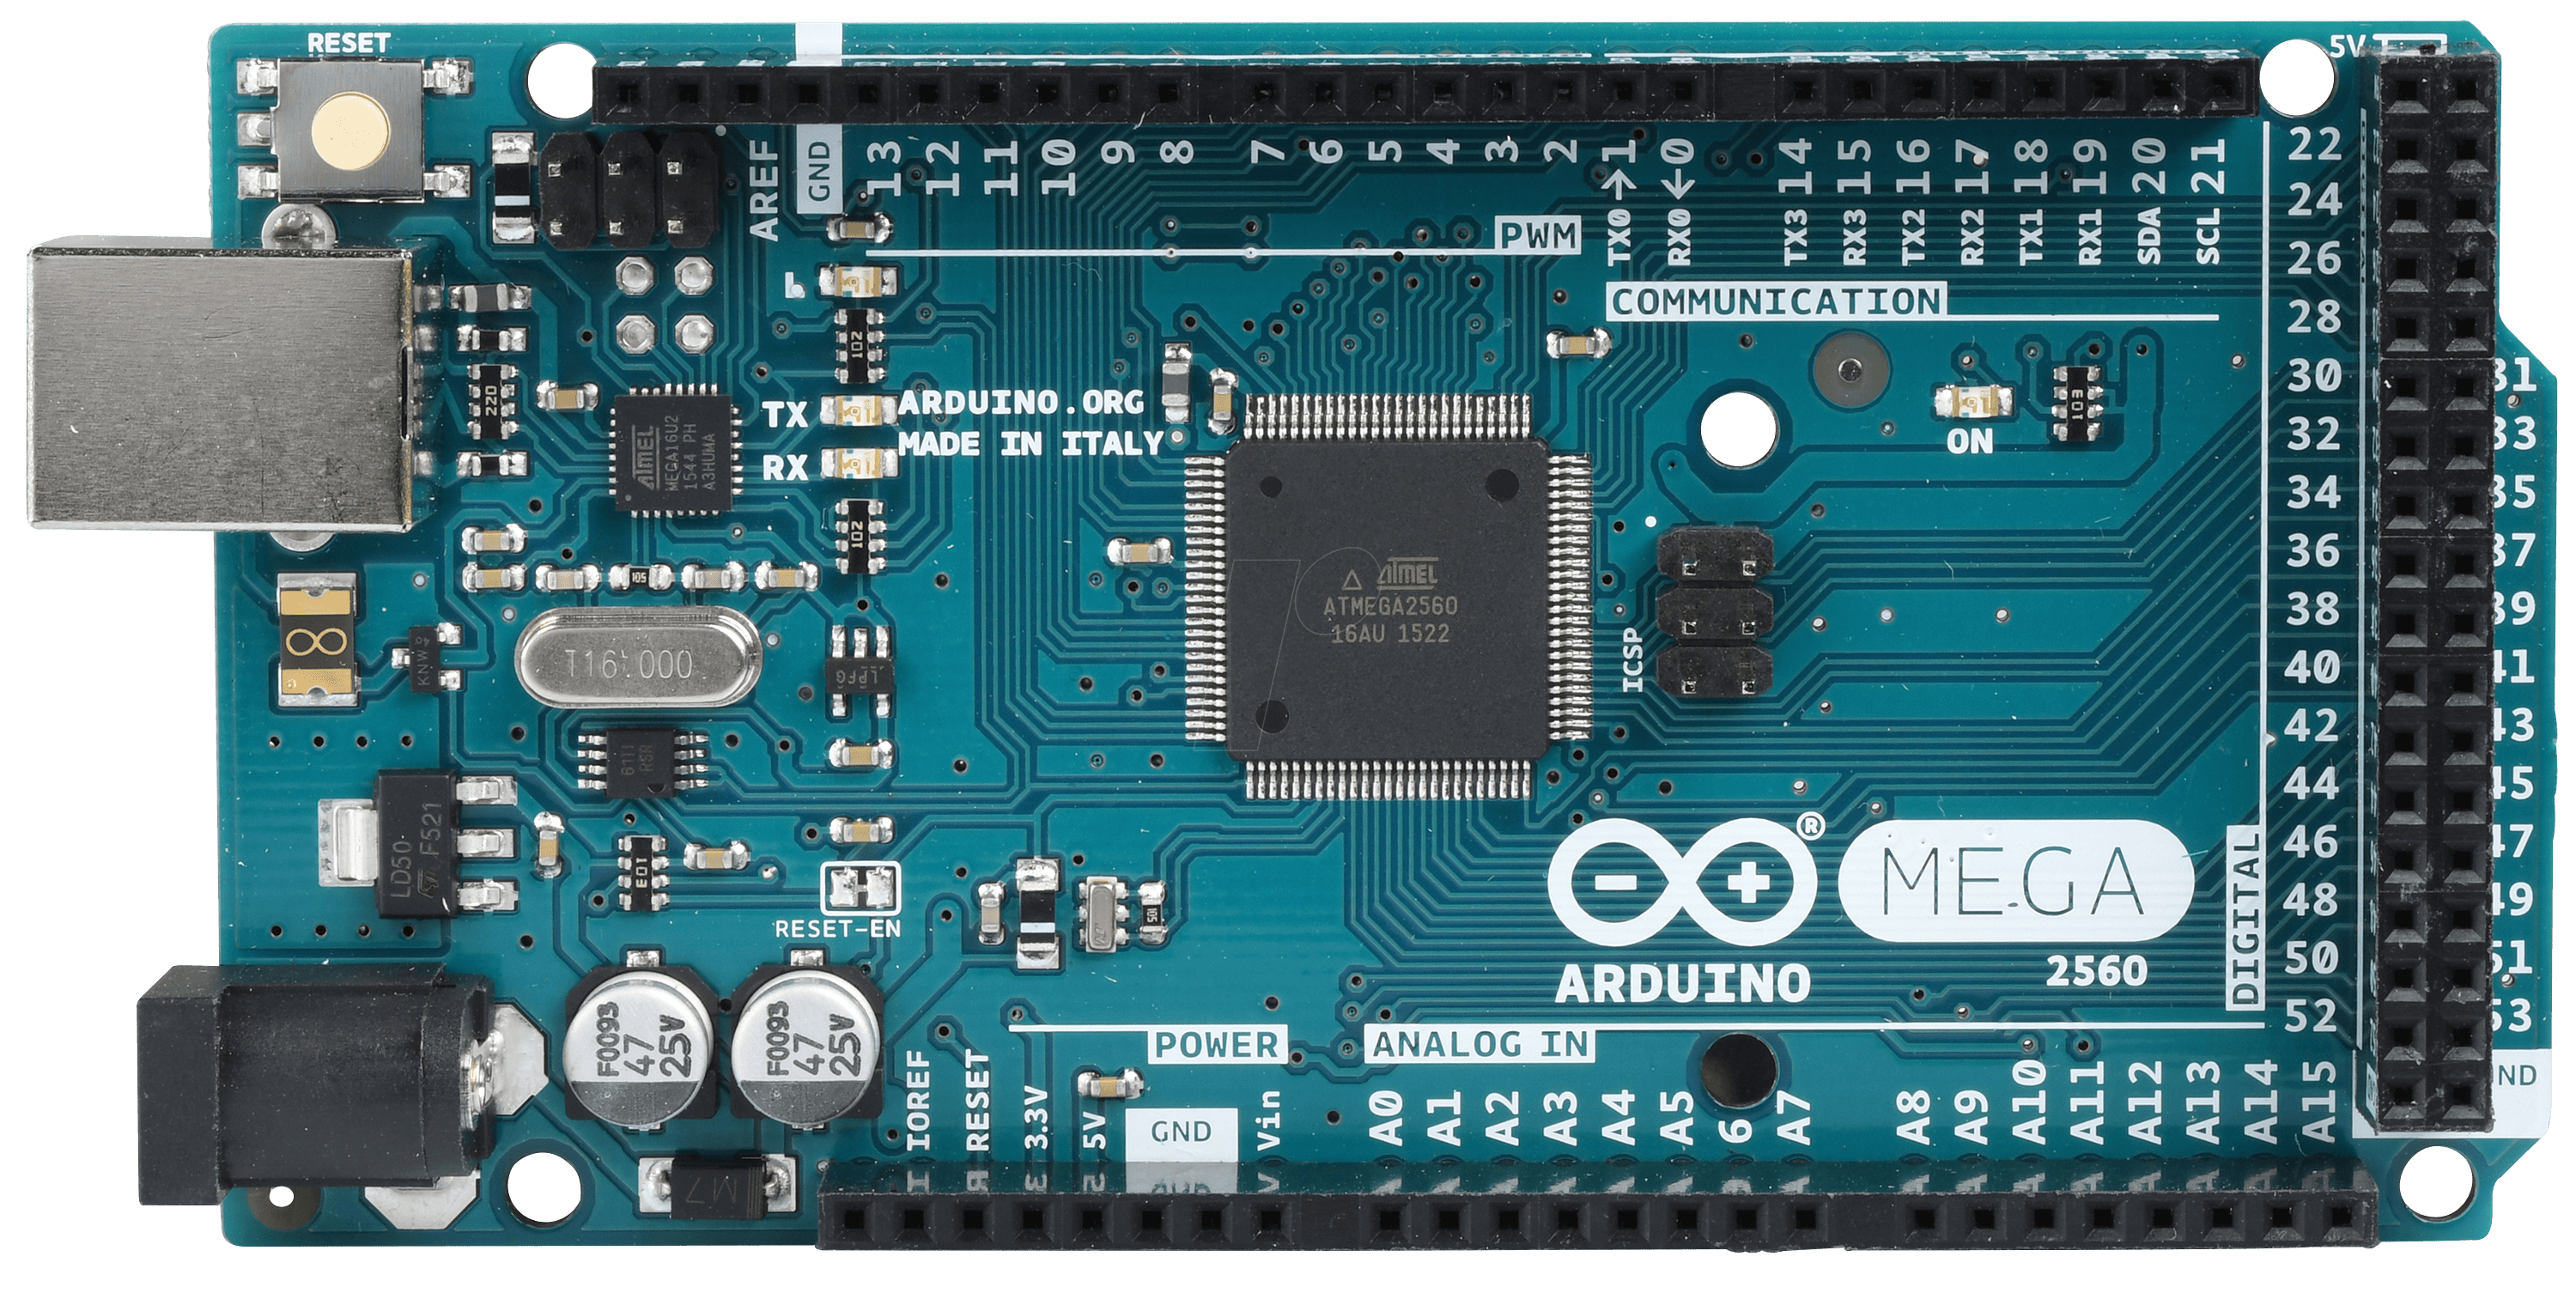
\includegraphics[width=0.5\textwidth]{rysKonstrukcja/Mega.png} & 
				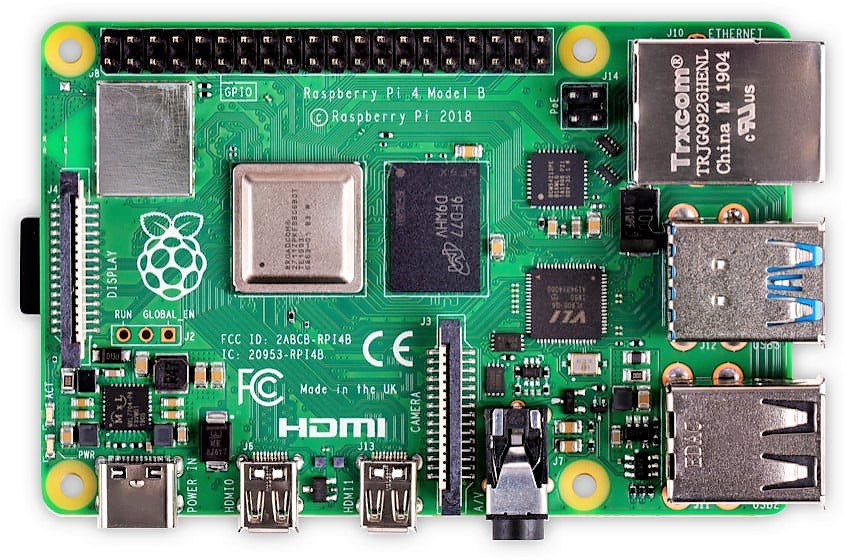
\includegraphics[width=0.5\textwidth]{rysKonstrukcja/raspberry.jpg} \\
			\end{tabular}
			\caption{Mikrokontrolery: a) Arduino Mega, b) Raspberry Pi}
			\label{fig:mikrokontrolery}
		\end{figure}
	
		Trzecią alternatywą łączącą pozytywy obu wymienionych wcześniej platform są mikrokontrolery STM32. Przykładową płytką jest STM32F103 Blue Pill \ref{fig:bluepillPlytka}. Posiada 32 konfigurowalne piny, 16 może obsługiwać zewnętrzne przerwania, 10 pinów połączonych z przetwornikiem ADC. Dodatkowo 18 może pracować z napięciem 5V (sam procesor pracuje na napięciu 3.3V) co może być przydatne zważywszy na fakt, że większa część gotowych modułów pracuje w logice 5V. Procesor wyposażony jest również w kontroler DMA, który pozwala na pomiary ADC oraz komunikację bez użycia procesora. Maksymalna nominalna częstotliwość taktowania wynosi 72MHz i dzięki pętli PLL może być łatwo konfigurowana. W przypadku niewielkiego braku mocy obliczeniowej istnieje możliwość łatwego overclockingu do 128MHz kosztem braku komunikacji przez USB. Procesor wyposażony jest także w 4 timery 16-bitowe, 4-kanałowe. Posiada także kilka możliwości wyboru API. Od wysokopoziomowego STM32duino, opartego na wspomnianym wcześniej Arduino, przez HAL oraz starsze SPL kończąc na systemie czasu rzeczywistego FreeRTOS \cite{FreeRTOS}. Ogromnym plusem jest niska cena. Płytka kosztuje około 1.5\$ (6zł).
	
		\begin{figure}[h]
			\centering
			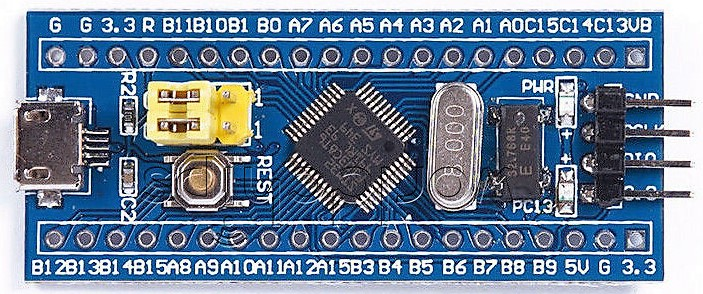
\includegraphics[width=0.8\textwidth]{rysKonstrukcja/bluepill.jpg} 
			\caption{Mikrokontroler STM32F103 Blue Pill}
			\label{fig:bluepillPlytka}
		\end{figure}
		
		Uwzględniając wskazane powyżej informacje wybrano płytkę STM32F103 Blue Pill. Zapewnia doby bilans między ilością peryferiów i wydajnością w porównaniu do pozostałych możliwości. Dodatkowo cechuje się najniższą ceną zakupu.
		
	\section{Pomiar odległości}
		
		Do orientacyjnego pomiaru odległości od przeszkód został wykorzystany moduł z czujnikiem ultradźwiękowym HC-SR04 \ref{fig:HCSR04}. Czujnik pozwala na pomiar odległości w zakresie \SI{2}{} --  \SI{400}{\centi\meter} z rozdzielczością \SI{0.3}{\centi\meter}. W trakcie projektowania brano pod uwagę, że na pomiar wpływa również propagacja fal dźwiękowych. Dlatego uwzględniono dodatkowe czujniki wykrywające przeszkody.
		
		\begin{figure}[H]
			\centering
			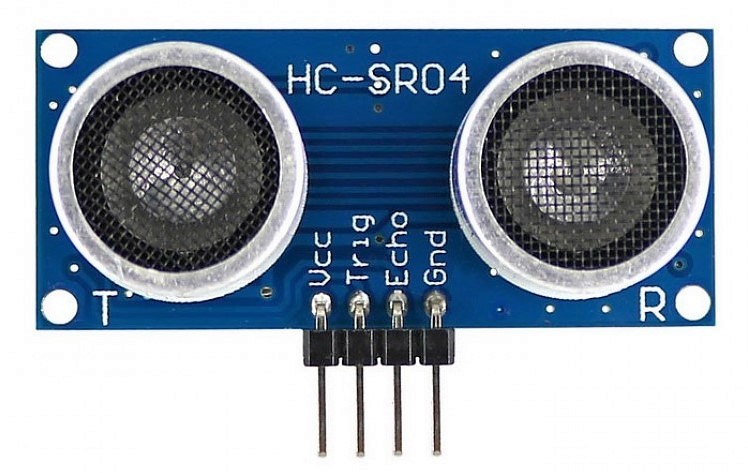
\includegraphics[width=0.4\textwidth]{rysKonstrukcja/HC-SR04.jpg} 
			\caption{Ultradźwiękowy moduł pomiaru odległości}
			\label{fig:HCSR04}
		\end{figure}
	
		Aby dokonać pomiaru czujnikiem należy na wejście Trig podać stan wysoki na co najmniej \SI{10}{\micro\second}. Moduł wysyła wtedy 8 ultradźwiękowych fal o częstotliwości \SI{40}{\kilo\hertz}. Po odebraniu pomiaru na pinie Echo pojawia się stan wysoki. W zależności od odległości od wykrytej przeszkody czas trwania wynosi od \SI{150}{\micro\second} do \SI{22}{\milli\second}. Jeśli nie wykryto przeszkody, czas stanu wysokiego wynosi \SI{38}{\milli\second}. Odległość w centymetrach można obliczyć korzystając z uproszczonej zależności \ref{eq:OdlegloscOdPrzeszkody}.
		
		\begin{equation}\label{eq:OdlegloscOdPrzeszkody}
			d = \unit[\frac{t}{58}]{cm}
		\end{equation}
		gdzie t - czas stanu wysokiego na pinie Echo w \SI{}{\micro\second}.	
		\textcolor{red}{dodać przebiegi z oscyloskopu}
	
	\section{Pomiar odległości od podłogi}
		Aby uniemożliwić robotowi wjazd w niebezpieczny obszar i tym samym zapobiec m.in. spadnięciu ze schodów. Zastosowano czujniki odbiciowe IR mierzące aktualną odległość od podłogi Rys \ref{fig:czujnikIR}. Czujnik ten ma wbudowany komparator LM393 regulowany potencjometrem. W przypadku detekcji zbyt dużej odległości na pin sygnałowy wystawiany jest odpowiedni stan logiczny. Dzięki temu nie ma potrzeby robienia pomiarów ADC oraz obsługi sprzętowej. Pozwala to dzięki mechanizmowi przerwań mikrokontrolera na praktycznie natychmiastową reakcję w przypadku wykrycia niebezpieczeństwa. 
		
		\begin{figure}[H]
			\centering
			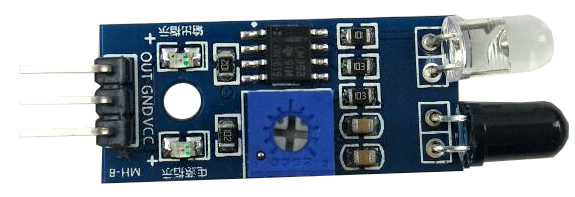
\includegraphics[width=0.6\textwidth]{rys02/czujnikIR.png} 
			\caption{Odbiciowy czujnik IR}
			\label{fig:czujnikIR}
		\end{figure}
	
	\section{Napęd}
		Jako napęd robota wykorzystano silniki szczotkowe DC z wbudowaną przekładnią. Parametry znamionowe silnika przedstawione są w tabeli \ref{tab:Napęd}.
		
		\begin{table}[H]
			\centering
			\begin{tabular}{|l|c|} \hline
				\textbf{Parametr} & Wartość \\
				\hline
				\hline  \textbf{Napięcie zasilania}& 3 -- \SI{6}{\volt}  \\
				\hline 	\textbf{Prędkość obrotowa po redukcji (\SI{6}{\volt})}& \SI{100}{RPM} \\
				\hline 	\textbf{Pobór prądu pod obciążeniem (\SI{6}{\volt})}& \SI{350}{\mA} \\
				\hline 	\textbf{Pobór prądu bez obciążenia (\SI{6}{\volt})}& \SI{170}{\mA} \\
				\hline 	\textbf{Siła ciągu na przekładni (\SI{6}{\volt})}& \SI[per-mode=symbol]{5,5}{\kg\per\cm} \\
				\hline
			\end{tabular}
			\caption{Parametry znamionowe silników napędowych}
			\label{tab:Napęd}
		\end{table}
	
		Do sterowania silnikami wykorzystano mostek H zbudowany w oparciu o układ L9110S. Pozwala on na sterowanie zarówno prędkością jak i kierunkiem obrotów silników niezależnie od siebie. Parametry znamionowe mostka przedstawione są w tabeli \ref{tab:MostekH}.
		
		\begin{table}[H]
			\centering
			\begin{tabular}{|l|c|} \hline
				\textbf{Parametr} & Wartość \\
				\hline
				\hline  \textbf{Napięcie zasilania}& 5 -- \SI{12}{\volt}  \\
				\hline 	\textbf{Maksymalne napięcie zasilania silników} & \SI{12}{\volt} \\
				\hline 	\textbf{Maksymalny prąd na kanał}& \SI{800}{\mA} \\
				\hline 	\textbf{Ilość kanałów}& 2 \\
				\hline 	\textbf{Poziom sygnałów sterujących mostkiem}& CMOS/TTL \\
				\hline
			\end{tabular}
			\caption{Parametry znamionowe mostka H}
			\label{tab:MostekH}
		\end{table}
	
		Sygnały jakie trzeba podać na wejście sterownika aby uzyskać pożądane sterowanie zostały przedstawione w tabeli \ref{tab:tabelaPrawdyMostkaH}.
		
		\begin{table}[H]
			\centering
			\begin{tabular}{|l|c|c|} \hline
				\textbf{1A} & 1B & Stan silnika \\
				\hline
				\hline 	0 & 0 & \textcolor{red}{Hamowanie silnikiem?}\\
				\hline 	1	& 0 & Do przodu \\
				\hline 	0 & 1 & Do tyłu \\
				\hline 	1 & 1 & \textcolor{red}{Hamowanie silnikiem?} \\
				\hline
			\end{tabular}
			\caption{Tabela prawdy mostka H}
			\label{tab:tabelaPrawdyMostkaH}
		\end{table}
		
		Silnik oraz mostek H przedstawione są na rysunku \ref{fig:silnikImostek}
		\begin{figure}[h]
			\centering
			\begin{tabular}{@{}ll@{}}
				a) & b) \\
				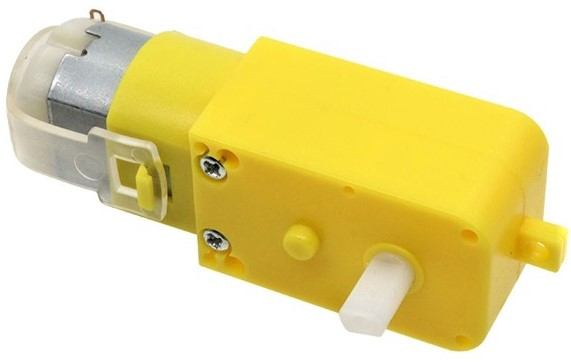
\includegraphics[width=0.5\textwidth]{rys02/silnikDC.jpg} & 
				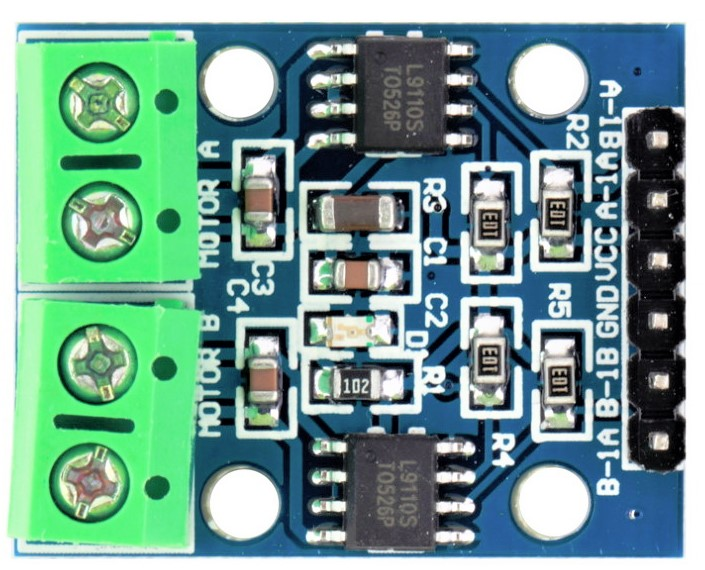
\includegraphics[width=0.4\textwidth]{rys02/mostekHzdj.jpg} \\
			\end{tabular}
			\caption{Zdjęcia: a) Silnika DC, b) Mostka H}
			\label{fig:silnikImostek}
		\end{figure}
	
		Do przeniesienia napędu wykorzystane zostały koła o średnicy \SI{68}{\milli\meter}. Przy maksymalnej prędkości obrotowej silnika robot osiąga prędkość wynoszącą w przybliżeniu \SI[per-mode=symbol]{3.56}{\cm\per\second}.
		
	\section{Rozpoznawanie pozycji}
		Do obliczania aktualnej pozycji i orientacji robota wykorzystanie zostały czujniki szczelinowe w połączeniu z płytkami szczelinowymi. Czujnik optyczny posiada wbudowany komparator LM393 dzięki czemu istnieje prosta możliwość detekcji czy sygnał optyczny jest odbierany czy nie. W połączeniu z płytką szczelinową mocowaną na wale silnika daje to prosty enkoder impulsowy. Płytka szczelinowa posiada rozdzielczość 20 linii na obrót. Obsługując impulsy w przerwaniach mikrokontrolera oraz wyzwalając przerwanie zarówno na zboczu narastającym jak i opadającym można osiągnąć rozdzielczość 40 impulsów na obrót. Uwzględniając średnicę koła niepewność pozycjonowania wynosi w przybliżeniu \SI{5.34}{mm}. Jest ona zbyt duża aby zapewnić precyzyjne sterowanie robotem. Dlatego zdecydowano się na zbudowanie przekładni zwiększającej ilość obrotów płytki enkodera. Przekładnia jest dwustopniowa z 5-krotnym wzmocnieniem w każdym ze stopni. Ostatecznie osiągamy 25-krotne zwiększenie prędkości obrotowej enkodera. Daje to nam 1000 impulsów na obrót i niepewność pozycjonowania wynoszącą w przybliżeniu \SI{0.21}{\milli\meter}. Czujnk szczelinowy wraz z płytką enkodera zostały przedstawione na rysunku \ref{fig:enkoderZplytka}.
		
		\begin{figure}[h]
			\centering
			\begin{tabular}{@{}ll@{}}
				a) & b) \\
				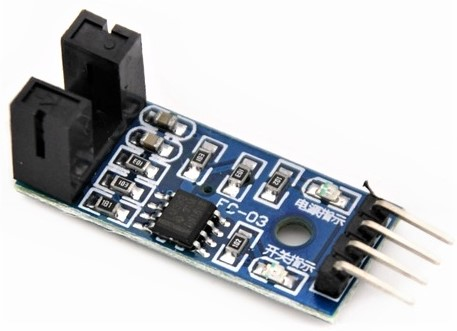
\includegraphics[width=0.5\textwidth]{rys02/enkoder.jpg} & 
				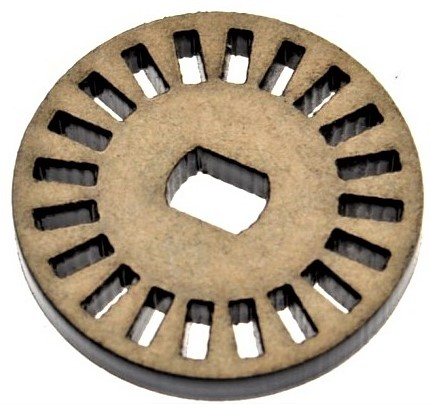
\includegraphics[width=0.2\textwidth]{rys02/plytkaEnkodera.jpg} \\
			\end{tabular}
			\caption{Zdjęcia: a) Czujnik szczelinowy, b) Płytka szczelinowa}
			\label{fig:enkoderZplytka}
		\end{figure}
	
	\section{Zasilanie}
	
		Jako zasilanie wykorzystanie 2 akumulatory Li-Ion 18650 połączone szeregowo. Napięcie nominalne takiego pakietu wynosi \SI{7.4}{\volt}. Przewagą takiego rozwiązania względem połączenia równoległego jest zmniejszenie prądów płynących w przewodach zasilających. Przyczyni się to do mniejszych strat na rezystancjach połączeń oraz zwiększy żywotność przełącznika bistabilnego On/Off. Aby dopasować napięcie do zasilania mikrokontrolera oraz peryferiów wykorzystano 2 przetwornice obniżające napięcie zbudowane w oparciu o układ MP2307. Jedna została wyregulowana na napięcie \SI{3.3}{\volt}, natomiast druga na \SI{5}{\volt}. Parametry techniczne przetwornic zostały przedstawione w tabeli \ref{tab:PrzetwornicaStepDown}.
		
		\begin{table}[H]
			\centering
			\begin{tabular}{|l|c|} \hline
				\textbf{Parametr} & Wartość \\
				\hline
				\hline  \textbf{Napięcie wejściowe}& 4.75 -- \SI{23}{\volt}  \\
				\hline 	\textbf{Napięcie wyjściowe} & 1 -- \SI{17}{\volt} \\
				\hline 	\textbf{Maksymalny prąd wyjściowy}& Szczytowy \SI{3}{\ampere}, ciągły \SI{1.8}{\ampere} \\
				\hline 	\textbf{Maksymalna sprawność konwersji}& \SI{98}{\percent} \\
				\hline 	\textbf{Częstotliwość przełączania}& \SI{340}{\kHz} \\
				\hline
			\end{tabular}
			\caption{Parametry znamionowe przetwornicy obniżającej napięcie}
			\label{tab:PrzetwornicaStepDown}
		\end{table}
	
		Baterie Li-Ion są bardzo wrażliwe zarówno na przeładowywanie \cite{ladowanieLiIon} jak i nadmierne rozładowanie \cite{rozladowywanieLiIon1, rozladowywanieLiIon2}. Najniższe napięcie rozładowania jakiego nie zaleca się przekraczać wynosi \SI{2.4}{\volt}, natomiast typową wartością eksploatacji jest \SI{3}{\volt} \cite{rozladowywanieLiIon2}. Z drugiej strony nadmierne przeładowywanie również drastycznie wpływa na żywotność akumulatorów. Nominalnym napięciem ładowania jest \SI{4.2}{\volt}. Jednak można ładować ogniwa do niższego napięcia zmniejsza się wtedy ich pojemność ale wzrasta żywotność. Wpływ końcowego napięcia ładowania na ogniwa przedstawiono w tabeli w oparciu o informacje ze źródła \cite{ladowanieLiIon}
		
		\begin{table}[H]
			\centering
			\begin{tabular}{|l|c|c|} \hline
				Napięcie końcowe \unit{V} & Ilość cykli rozładowywania & Pojemność ogniwa \\
				\hline
				\hline \SI{4.30}{\volt} & 150 -- 200 & 110 -- \SI{115}{\percent}\\
				\hline \SI{4.25}{\volt}	& 200 -- 350 & 105 -- \SI{110}{\percent}\\
				\hline \SI{4.20}{\volt}	& \textcolor{red}{300 -- 500} & \SI{100}{\percent}\\
				\hline \SI{4.15}{\volt}	& 400 -- 700 & 90 -- \SI{95}{\percent} \\
				\hline \SI{4.10}{\volt}	& 600 -- 1000 & 85 -- \SI{90}{\percent}\\
				\hline \SI{4.05}{\volt} & 850 -- 1500 & 80 -- \SI{85}{\percent}\\
				\hline \SI{4.00}{\volt} & 1200 -- 2000 & 70 -- \SI{75}{\percent}\\
				\hline
			\end{tabular}
			\caption{Wpływ napięcia końcowego na żywotność akumulatorów Li-Ion}
			\label{tab:napięcieKońcoweLiIon}
		\end{table}
	
%%%
%%%Uwaga: tytuł powinien zmieścić się w okienku kolorowej okładki (którą
%%%powinna dostarczyć uczelniana administracja). Proszę posterować
%%%parametrami, aby "wpasować" w okienko własny tekst.
%%%
%%%Do ASAPa należy wprowadzić pracę dyplomową/projekt inżynierski w pliku o nazwie:
%%%
%%%W04_[nr albumu]_[rok kalendarzowy]_[rodzaj pracy] (szczegółowa instrukcja pod adresem asap.pwr.edu.pl)
%%%
           %%%Przykładowo:
        %%%­W04_123456_2015_praca inżynierska.pdf     - praca dyplomowa inżynierska
        %%%W04_123456_2015_projekt inżynierski.pdf   - projekt inżynierski
        %%%W04_123456_2015_praca magisterska.pdf  - praca dyplomowa magisterska
%%%
              %%%rok kalendarzowy ? rok realizacji kursu „Praca dyplomowa” (nie rok obrony) 